\documentclass[11pt]{article}

\usepackage[utf8]{inputenc}
\usepackage{amsmath}
\usepackage{amsfonts}
\usepackage{mathtools}
\usepackage{geometry}
\usepackage{graphicx}
\usepackage[colorlinks=true, linkcolor=blue, urlcolor=blue]{hyperref}
\usepackage{titling}
\usepackage[skip=10pt plus1pt]{parskip}


\newcommand{\subtitle}[1]{%
  \posttitle{%
    \par\end{center}
    \begin{center}\large#1\end{center}
    \vskip0.5em}%
}

\setlength{\parindent}{0pt}

\title{Spotify Music Clustering}
\subtitle{DS 3000 Mini-Project Report}
\author{Dylan McCormick\\\href{mailto:mccormick.dy@northeastern.edu}{mccormick.dy@northeastern.edu} \and Ali Salha\\\href{mailto:salha.a@northeastern.edu}{salha.a@northeastern.edu}}
\date{April 18, 2026}

\geometry{margin=1in}
\graphicspath{{./images/}}

\begin{document}
\maketitle

\textbf{Group Name:} Tarboosh Shawarma Data Analysis Group\\
\textbf{Group Members:} Dylan McCormick, Ali Salha

\section{Domain: Spotify Music}

We wanted to see how we could apply the concepts learned in Foundations of Data Science to a domain that we are both passionate about: music. We found a vast dataset of Spotify songs online, and since we both held a keen interest in machine learning, we figured that we could use the features of the dataset in a way such that we could cluster songs together based on their features.

\subsection{Data}
\label{sec:data}

We used the \href{https://www.kaggle.com/datasets/maharshipandya/-spotify-tracks-dataset}{Spotify Tracks Dataset} from Kaggle, which contains approximately 90,000 unique songs with their features. The dataset is comprehensive, containing various features such as acousticness, danceability, energy, instrumentalness, loudness, etc. which are all numerical values that have been methodically extracted from the audio files of the songs and ranged between 0 and 1. Also, there were some categorical features (such as whether the song is explicit or not) that we mapped to an integer value (0 or 1) to make them a numeric value we could use in our clustering algorithm.

The feature columns we used for our dataset are as follows: danceability, energy, loudness, tempo, valence, acousticness, instrumentalness, speechiness, liveness, duration\_ms, mode, time\_signature, and explicit.

\subsection{Question}

The primary question we were looking to address for this project was: \textit{Are there a small number of underlying, generalized “types” of songs?} We wanted to see if we could cluster songs together based on their features, and if so, what are the optimal clusters.

\section{DS 3000 Concepts}

To answer our question, we applied the following techniques and concepts from DS 3000:

\begin{itemize}
    \item \textbf{Principal Component Analysis (PCA):} We used PCA to reduce the dimensionality of our dataset while retaining a set amount of variance. This allowed us to work with a more manageable number of features while still capturing the essence of the data. Also, we wanted to see if we could use the first two principal components to visualize the clusters of songs in a 2D space.
    \item \textbf{Optimization (K-Means Clustering):} Although K-Means Clustering is not a concept that we explicitly covered in DS 3000, we figured that since it uses the concept of optimization to find the optimal clusters for the dataset, it would be a valid technique to apply to our object. Also, the whole backbone of K-Means clustering is based on norms and distances, so we thought it would be a good way to apply the concepts of norms and distances that we learned in DS 3000.
    \item \textbf{Norms and Distances:} As mentioned before, norms and distances are the backbone of K-Means clustering, so we indirectly dealt with norms and distances when we applied K-Means clustering to our dataset. K-Means clustering uses the L2 norm (Euclidean distance) to measure the distance between data points and cluster centroids in our K-Means algorithm.
\end{itemize}

\section{Applying Concepts}

The following subsections detail how we applied the above concepts to our dataset.

\subsection{Principal Component Analysis (PCA)}

But first, \textit{why did we even choose to apply PCA to our dataset?} Besides trying to create a visualization of the clusters in a 2D space, a smaller impact of principal component analysis is that it can help to reduce the noise in our dataset by only capturing the most important features that explain the variance in our dataset.

\subsubsection{Z-Score Standardization}

Before applying PCA, we first had to standardize our dataset using z-scores. Despite our data being already normalized between 0 and 1, this doesn't necessarily mean that all of our features were on the same scale, especially if a specific feature didn't actually have a range between 0 and 1. Also, it is just good practice to standardize our dataset, especially if we want to change the data to a non-standardized dataset in the future. So, we used the following formula to standardize our dataset:

\begin{equation}
    z = \frac{x - \mu}{\sigma}
\end{equation}
where:
\begin{tabular}{ll}
    $x$ & is the original value of the feature \\
    $\mu$ & is the mean of the feature \\
    $\sigma$ & is the standard deviation of the feature
\end{tabular}

\subsubsection{Covariance Matrix}

After standardizing our dataset, we then computed the covariance matrix of our dataset. This would just show us how much the features in our dataset vary together. Note that since our dataset is standardized, the covariance matrix is basically the same as the correlation matrix, since the standard deviation of each feature is 1.

The covariance of two features $x_1$ and $x_2$ is calculated using the following formula:

\begin{equation}
    cov(x1, x2) = \frac{\sum_{i = 1}^{n}(x_{1_i} - \mu_1)(x_{2_i} - \mu_2)}{n - 1}
\end{equation}
where:
\begin{tabular}{ll}
    $x_{1_i}$ & is the value of the first feature for the $i$-th data point \\
    $x_{2_i}$ & is the value of the second feature for the $i$-th data point \\
    $\mu_1$ & is the mean of the first feature \\
    $\mu_2$ & is the mean of the second feature \\
    $n$ & is the number of data points
\end{tabular}

Let's take a look at the covariance matrix of our dataset. See section \hyperref[sec:data]{1.1 Data} for the order of the features in our dataset.
\setcounter{MaxMatrixCols}{13}
$$
C = \resizebox{\textwidth}{!}{$\begin{bmatrix}
1.00 & 0.13 & 0.26 & -0.05 & 0.48 & -0.17 & -0.19 & 0.11 & -0.13 & -0.07 & -0.07 & 0.21 & 0.12 \\
0.13 & 1.00 & 0.76 & 0.25 & 0.26 & -0.73 & -0.18 & 0.14 & 0.18 & 0.06 & -0.08 & 0.19 & 0.10 \\
0.26 & 0.76 & 1.00 & 0.21 & 0.28 & -0.59 & -0.43 & 0.06 & 0.08 & 0.00 & -0.04 & 0.19 & 0.11 \\
-0.05 & 0.25 & 0.21 & 1.00 & 0.08 & -0.21 & -0.05 & 0.02 & 0.00 & 0.02 & 0.00 & 0.07 & 0.00 \\
0.48 & 0.26 & 0.28 & 0.08 & 1.00 & -0.11 & -0.32 & 0.04 & 0.02 & -0.15 & 0.02 & 0.13 & 0.00 \\
-0.17 & -0.73 & -0.59 & -0.21 & -0.11 & 1.00 & 0.10 & 0.00 & -0.02 & -0.10 & 0.10 & -0.18 & -0.09 \\
-0.19 & -0.18 & -0.43 & -0.05 & -0.32 & 0.10 & 1.00 & -0.09 & -0.08 & 0.12 & -0.05 & -0.08 & -0.10 \\
0.11 & 0.14 & 0.06 & 0.02 & 0.04 & 0.00 & -0.09 & 1.00 & 0.21 & -0.06 & -0.05 & 0.00 & 0.31 \\
-0.13 & 0.18 & 0.08 & 0.00 & 0.02 & -0.02 & -0.08 & 0.21 & 1.00 & 0.01 & 0.01 & -0.02 & 0.03 \\
-0.07 & 0.06 & 0.00 & 0.02 & -0.15 & -0.10 & 0.12 & -0.06 & 0.01 & 1.00 & -0.04 & 0.02 & -0.07 \\
-0.07 & -0.08 & -0.04 & 0.00 & 0.02 & 0.10 & -0.05 & -0.05 & 0.01 & -0.04 & 1.00 & -0.02 & -0.04 \\
0.21 & 0.19 & 0.19 & 0.07 & 0.13 & -0.18 & -0.08 & 0.00 & -0.02 & 0.02 & -0.02 & 1.00 & 0.04 \\
0.12 & 0.10 & 0.11 & 0.00 & 0.00 & -0.09 & -0.10 & 0.31 & 0.03 & -0.07 & -0.04 & 0.04 & 1.00
\end{bmatrix}$}
$$

Lot to unpack here. This was computed using \texttt{np.cov(X\_scaled)}, but it uses the covariance formula. Also, notice that the diagonal of the covariance matrix is all 1s, and it is a symmetric matrix, which makes intuitive sense (the covariance of a feature with itself is just the variance of that feature, which is 1 since we standardized our dataset, and the covariance of feature A with feature B is the same as the covariance of feature B with feature A). I already noticed in this matrix that there are some features that have a high covariance with each other (such as energy and loudness, which have a covariance of 0.76), which makes sense since they are both related to the intensity of the song. Also, there are some features that have a negative covariance with each other (such as acousticness and energy, which have a covariance of -0.73), which also makes sense since they are inversely related (a song that is more acoustic is likely to be less energetic).

\subsubsection{Eigendecomposition}
After computing the covariance matrix, PCA then performs eigendecomposition on the covariance matrix to find the eigenvalues and eigenvectors. The eigenvalues represent the amount of variance explained by each principal component, while the eigenvectors represent the direction of the principal components in the original feature space. For the purposes of keeping this report concise, I will just provide the eigenvalues. The eigenvalues are as follows, truncated to 2 decimal places:
$$\lambda = \begin{bmatrix}
0.23 & 0.11 & 0.10 & 0.08 & 0.07 & 0.07 & 0.06 & 0.06 & 0.05 & 0.04 & 0.03 & 0.02 & 0.01
\end{bmatrix}$$

We set \textit{90\%} as our threshold for the amount of variance we wanted to retain in our dataset, which meant that we would need to keep the first 10 principal components. So, we did that, and the PCA transformation has been complete. Note that "Explained Variance Ratio" is just the eigenvalues divided by the sum of eigenvalues, which gives us the proportion of variance explained by each principal component.

\begin{figure}[h]
    \centering
    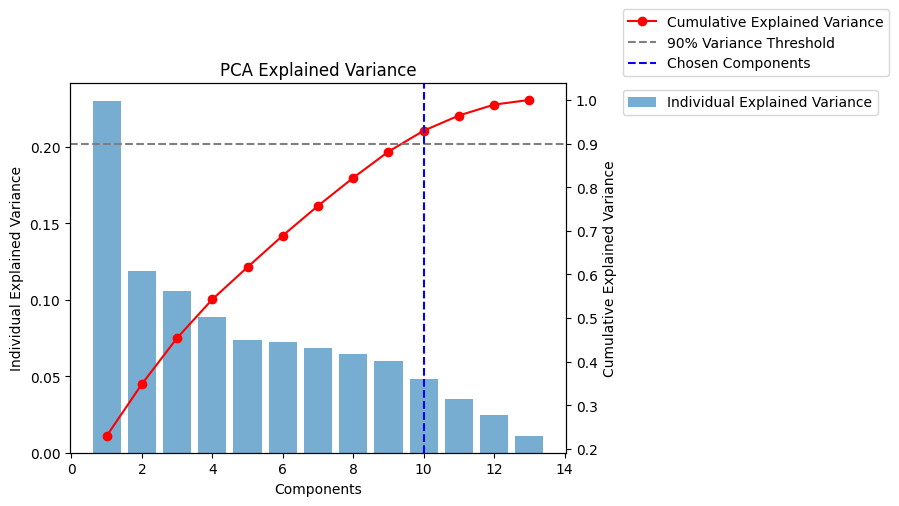
\includegraphics[width=1\textwidth]{pca_explained_variance.png}
    \caption{(Cumulative) Explained Variance Ratio of the Principal Components}
    \label{fig:pca_explained_variance}
\end{figure}

\subsection{Optimization (K-Means Clustering) \& Norms and Distances}

I have combined the two concepts of optimization and norms and distances into one section since it's hard to explain one without the other. K-Means clustering is a very simple optimization algorithm that tries to find the centroids of the optimal clusters in our dataset. The way it does this is by initializing $k$ random centroids, then assigning each data point to the nearest centroid (using the L2 norm), then updating the centroids by taking the mean of the data points assigned to each centroid, and then repeating this process until convergence (when the centroids do not change anymore). The objective function that K-Means tries to minimize is the sum of squared distances between each data point and its assigned centroid, which is given by the following formula. Note that the loss function we are trying to minimize is the within-cluster sum of squares (WCSS), which is the sum of squared distances between each data point and its assigned centroid. The WCSS is given by the following formula (see next page):

\pagebreak
\begin{equation}
    \underset{\mu_1, \dots, \mu_k}{\text{min}} \quad J = \sum_{i=1}^{n} \sum_{j=1}^{k} r_{ij} ||x_i - \mu_j||^2
\end{equation}
where:
\begin{tabular}{ll}
    $n$ & is the number of data points \\
    $k$ & is the number of clusters \\
    $r_{ij}$ & is a binary variable that is 1 if data point $i$ is assigned to cluster $j$, and 0 otherwise \\
    $x_i$ & is the $i$-th data point \\
    $\mu_j$ & is the centroid of cluster $j$ \\
    $||x_i - \mu_j||^2$ & is the squared L2 norm (Euclidean distance) between data point $i$ and centroid $j$
\end{tabular}

\subsubsection{Elbow Method}
To find the optimal number of clusters for our dataset, we used the elbow method, which involves plotting the within-cluster sum of squares (WCSS) for different values of $k$ and looking for the "elbow" point where the rate of decrease in WCSS slows down. Also referred to as "inertia" in the \texttt{sklearn.cluster.KMeans} implementation, we found the optimal number of clusters to be 6, as plotted below.

\begin{figure}[h]
    \centering
    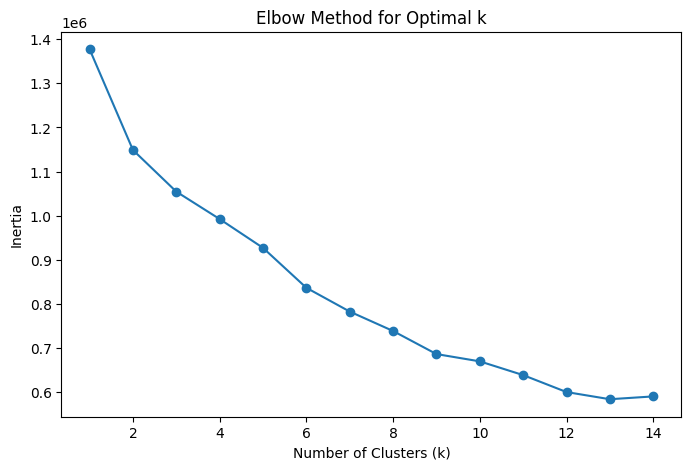
\includegraphics[width=.8\textwidth]{elbow_method_for_optimal_k.png}
    \caption{Elbow Method for Finding Optimal Number of Clusters}
    \label{fig:elbow_method}
\end{figure}

Now that we have found the optimal number of clusters, we can fit our K-Means model to our dataset and find the centroids of the clusters. We can also visualize the clusters in a 2D space using the first two principal components from our PCA transformation.

(see next page)

\pagebreak
\section{Conclusion}

We are trying to attack the question of whether there are a small number of underlying, generalized "types" of songs (that go beyond just genre). By analyzing this data using techniques such as PCA and K-Means clustering, the short answer is: \textit{yes}.

Long answer: We had to verify the resulting clusters had meaningful data that clearly abstract them from one-another. For example, if we had two clusters that were very similar to each other, like "Hype Music" and "Energetic Music", then we would have to question whether any of our clusters are even meaningful at all. To verify the assertion that our clusters are meaningful, we the cluster to each song and then looked at the mean of each feature for each cluster.

\begin{table}[h]
\centering
\resizebox{\textwidth}{!}{%
\begin{tabular}{ccccccccccccc c}
\hline
\textbf{Cluster} & \textbf{Danceability} & \textbf{Energy} & \textbf{Loudness} & \textbf{Tempo} & \textbf{Valence} & \textbf{Acousticness} & \textbf{Instrumentalness} & \textbf{Speechiness} & \textbf{Liveness} & \textbf{Duration\_ms} & \textbf{Mode} & \textbf{Time\_sig} & \textbf{Explicit} \\
\hline
0 & 0.44 & 0.82 & -5.53 & 142.35 & 0.40 & 0.13 & 0.05 & 0.09 & 0.36 & 241551.50 & 0.82 & 3.91 & 0.00 \\
1 & 0.42 & 0.24 & -15.87 & 108.29 & 0.27 & 0.82 & 0.35 & 0.05 & 0.17 & 211796.07 & 0.72 & 3.64 & 0.00 \\
2 & 0.65 & 0.65 & -7.13 & 117.36 & 0.63 & 0.31 & 0.02 & 0.07 & 0.17 & 209831.47 & 1.00 & 3.97 & 0.00 \\
3 & 0.64 & 0.71 & -6.56 & 120.34 & 0.57 & 0.22 & 0.03 & 0.08 & 0.19 & 221791.67 & 0.00 & 3.97 & 0.00 \\
4 & 0.59 & 0.74 & -8.67 & 126.88 & 0.33 & 0.09 & 0.78 & 0.07 & 0.17 & 319245.62 & 0.52 & 3.95 & 0.00 \\
5 & 0.64 & 0.72 & -6.59 & 121.39 & 0.47 & 0.23 & 0.05 & 0.21 & 0.25 & 203524.77 & 0.58 & 3.95 & 0.97 \\
\hline
\end{tabular}%
}
\caption{Mean Feature Values per Cluster}
\label{tab:cluster_means}
\end{table}

Manually analyzing the data, we synthesized the following descriptions for each cluster:

\begin{enumerate}
    \setcounter{enumi}{-1}
    \setlength{\parskip}{0pt}
    \item \textbf{Hype/Live} --- High energy, highest loudness, fastest tempo, not really acoustic or instrumental, high speechiness (comparison excludes cluster 5). Could be good for concerts.
    \item \textbf{Chill/Acoustic} --- Low energy, most quiet, slowest tempo, highest acousticness, very instrumental (excluding cluster 4), lowest speechiness, not very lively.
    \item \textbf{Feel-Good} --- Highest danceability, high energy, 2nd loudest, high tempo, not very instrumental, but has a mode average of 1.0 (major key).
    \item \textbf{Moody/Dance} --- Similar to cluster 2 but has a darker or more emotional tone, as told by the mode average of 0.0 (minor key).
    \item \textbf{Instrumental} --- Focuses more on the instruments rather than vocality of the track (has the lowest speechiness). Probably classical, ambient, or electronic instrumental tracks.
    \item \textbf{Rap/Explicit} --- Almost entirely explicit, probably rap, also very speechy and energetic.
\end{enumerate}

We can definitely say that there are a small number of underlying, \textit{distinct} types of songs, and that these types of songs go beyond just genre. For example, we have a "Hype/Live" cluster that could contain songs from various genres (rock, pop, hip-hop, etc.) but they all share the common characteristics of being high energy, loud, and fast tempo. We also have a "Chill/Acoustic" cluster that could contain songs from various genres (folk, indie, acoustic pop, etc.) but they all share the common characteristics of being low energy, quiet, slow tempo, and acoustic. So, we can definitely say that there are a small number of underlying, distinct types of songs that go beyond just genre.

\end{document}